%% V1.0
%% by Gabriel Garcia, gabrcg@gmail.com
%% This is a template for Udacity projects using IEEEtran.cls

%% Be Udacious!

\documentclass[10pt,journal,compsoc]{IEEEtran}

\usepackage[pdftex]{graphicx}    
\usepackage{cite}
\hyphenation{op-tical net-works semi-conduc-tor}
\usepackage{hyperref}
\usepackage{listings}


\begin{document}

\title{Where am I?}

\author{Jeremy Hale}

\markboth{Localization project, Robotics Nanodegree Program, Udacity}%
{}
\IEEEtitleabstractindextext{%

\begin{abstract}
For the Udacity Robotics Nanodegree Where Am I? localization project, two different robot models were constructed in URDF and made to navigate a simple map. Both robots use a camera and a laser scanner as inputs and use differential drive for locomotion, however, their configuration is significantly different. The simulation was carried out using ROS, Gazebo, and RViz.
\end{abstract}

% Note that keywords are not normally used for peerreview papers.
\begin{IEEEkeywords}
Robot, IEEEtran, Udacity, \LaTeX, Localization.
\end{IEEEkeywords}}


\maketitle
\IEEEdisplaynontitleabstractindextext
\IEEEpeerreviewmaketitle
\section{Introduction}
\label{sec:introduction}

\IEEEPARstart{T}{he} project is an exercise in defining robots within ROS, but more importantly, an exercise is localization. Localization is a key topic in robotics and important for student understanding. While there are several types of localization problems, this project deals with localization when the map is known but the location must be determined using sensors.

\section{Background}
As per the project instructions, Adaptive Monte Carlo Localization module in ROS was used as well as the ROS Navigation stack.

\subsection{Kalman Filters}
At a high-level, a Kalman filter takes multiple, related, noisy sensor readings and combines them into one estimation that has less randomness than any of the individual readings.

Linear Kalman filters are based on gaussian distributions, and their validity is limited to linear state transitions. Extended Kalman filters use a linear approximation (Taylor series) to allow non-linear functions.

\subsection{Particle Filters}
A particle filter consists of two stages: a transformation/measurement stage and a resampling stage. Initially, particles are randomly distributed. The particles are transformed based on some input (motion for example), then based on the measurement, particles with a high probability of having the same measurement have their weight increased. During the 2nd stage, resampling, particles with large weights are retained while those with low weights are discarded.

After several cycles, the particles converge on the estimated location.

\subsection{Comparison / Contrast}
MCL is easy to implement, is not restricted to Gaussian sensor noise, and is more flexible in terms of computational resources.

\section{Simulations}
Both the benchmark robot and the personal robot reached the navigation goals successfully using the same parameters. 

The personal model is shown below. The robot is supposed to look like R2D2. Compared to the Udacity robot, the student robot is larger and tilted back at 30 degrees. The camera is no longer horizontal, however the laser scanner was kept horizontal.

Some inspiration was taken from the udacity xacro file as well as the ROS URDF tutorials (
\url{https://github.com/ros/urdf_tutorial/tree/master/urdf}
).

\begin{figure}[thpb]
      \centering
      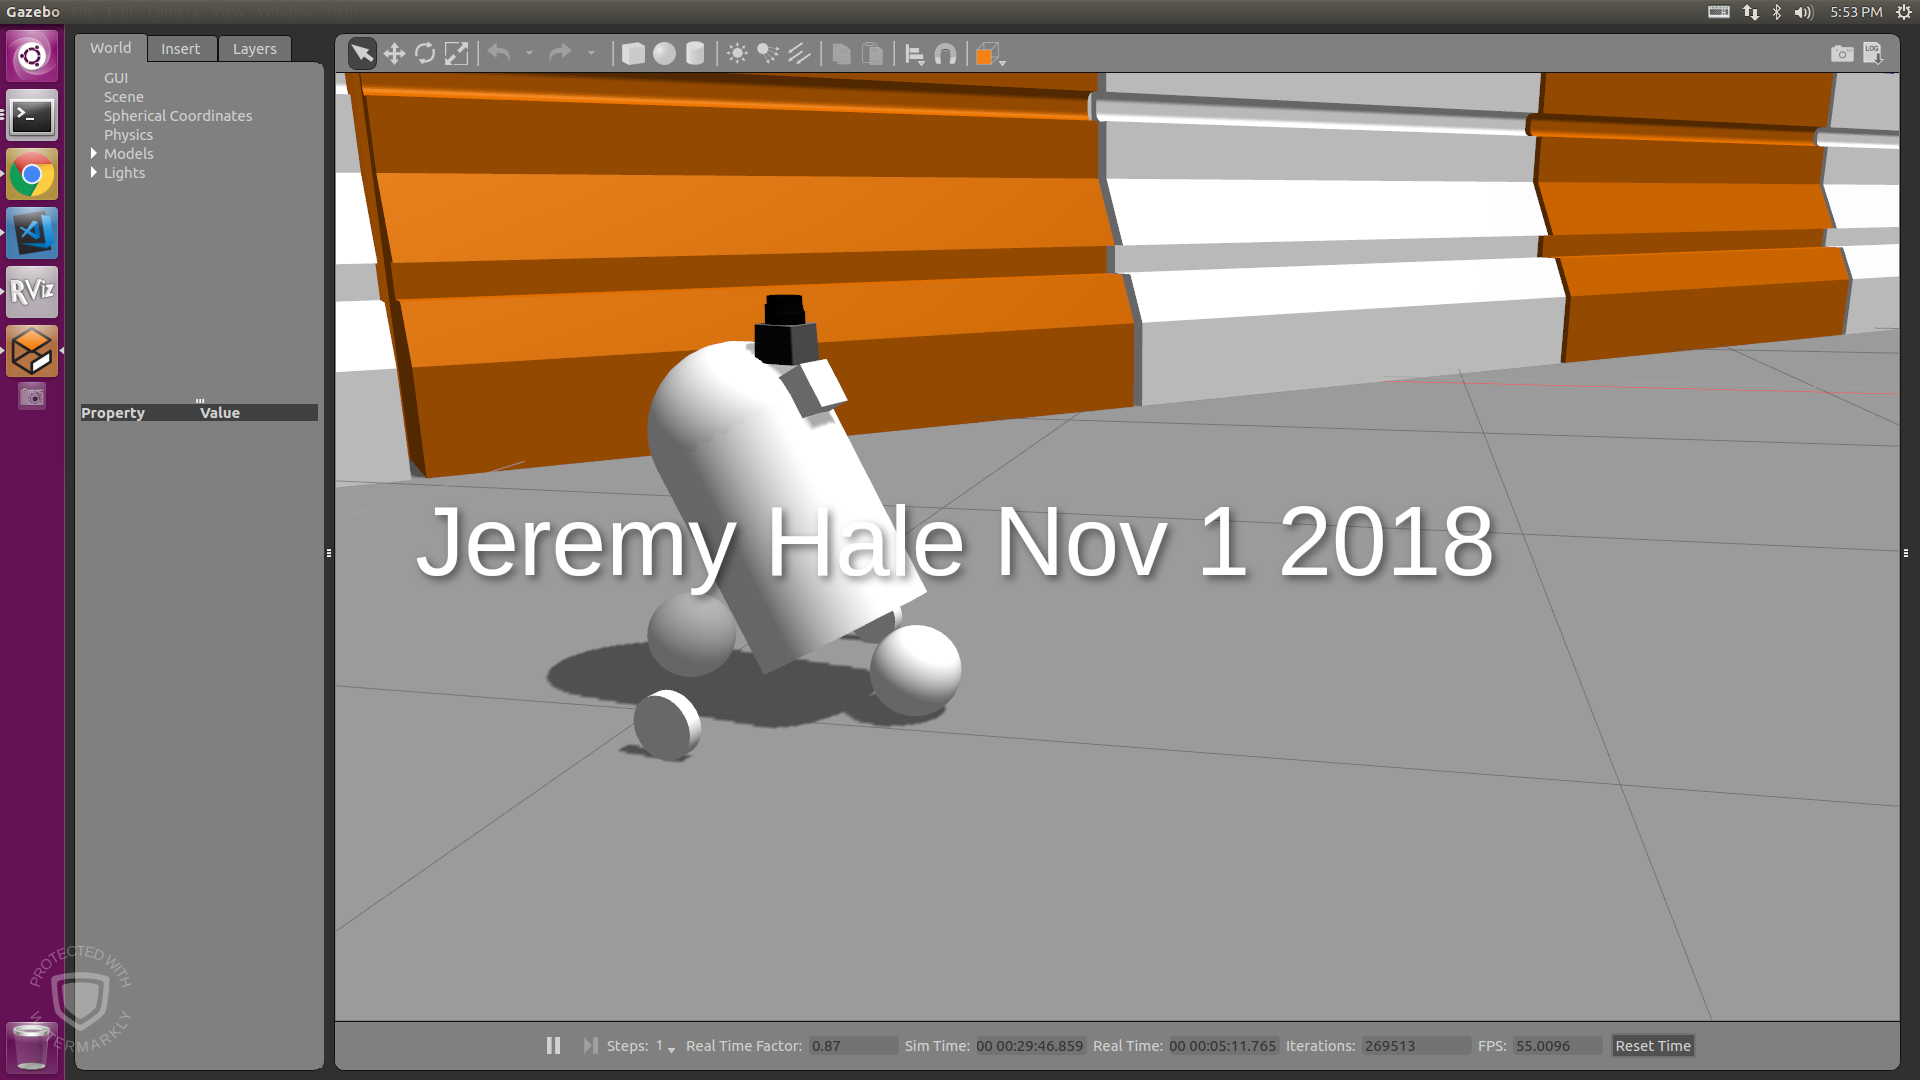
\includegraphics[width=\linewidth]{my_bot_gazebo}
      \caption{My Robot Gazebo}
      \label{fig:robot1}
\end{figure}


The Udacity provided robot successfully navigates to the goal.
\begin{figure}[thpb]
      \centering
      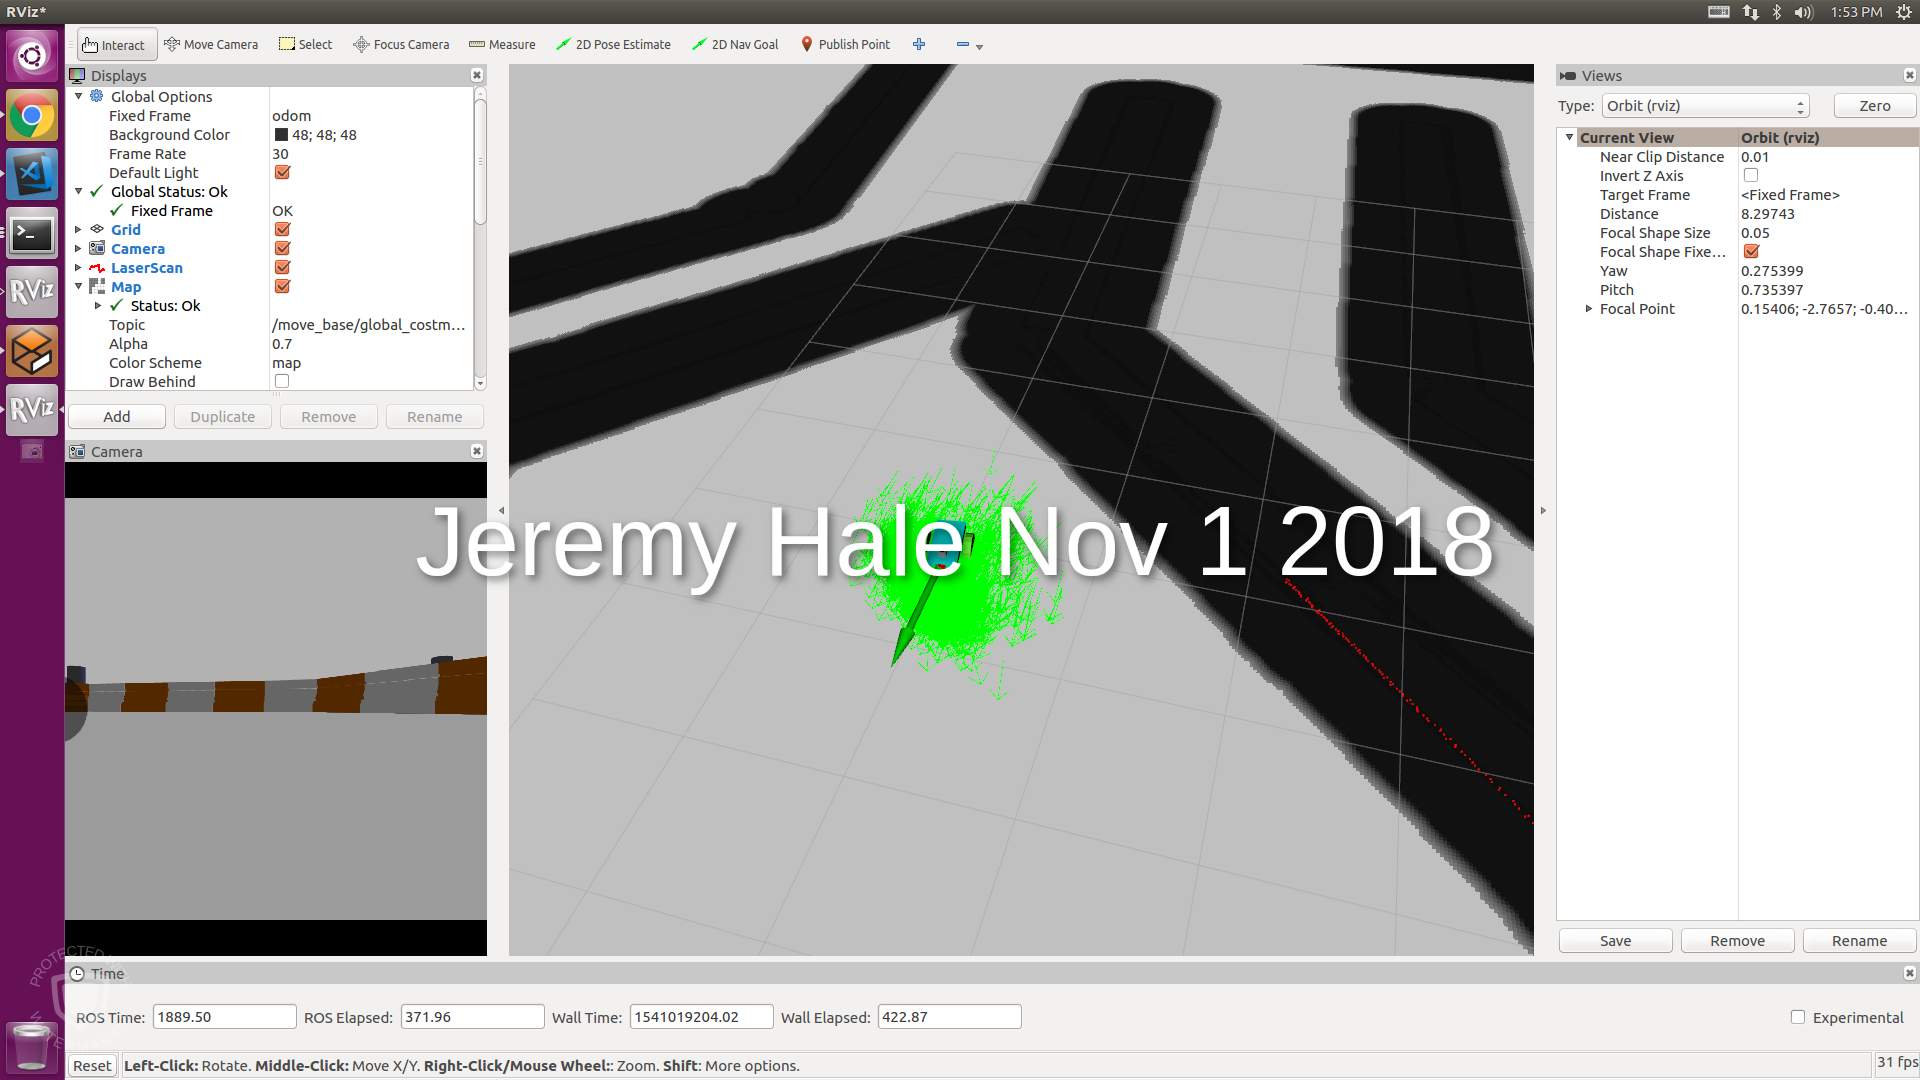
\includegraphics[width=\linewidth]{udacity_bot_goal_close}
      \caption{Udacity Robot}
      \label{fig:robot2}
\end{figure}

The student-defined robot successfully navigates to the goal.

\begin{figure}[thpb]
      \centering
      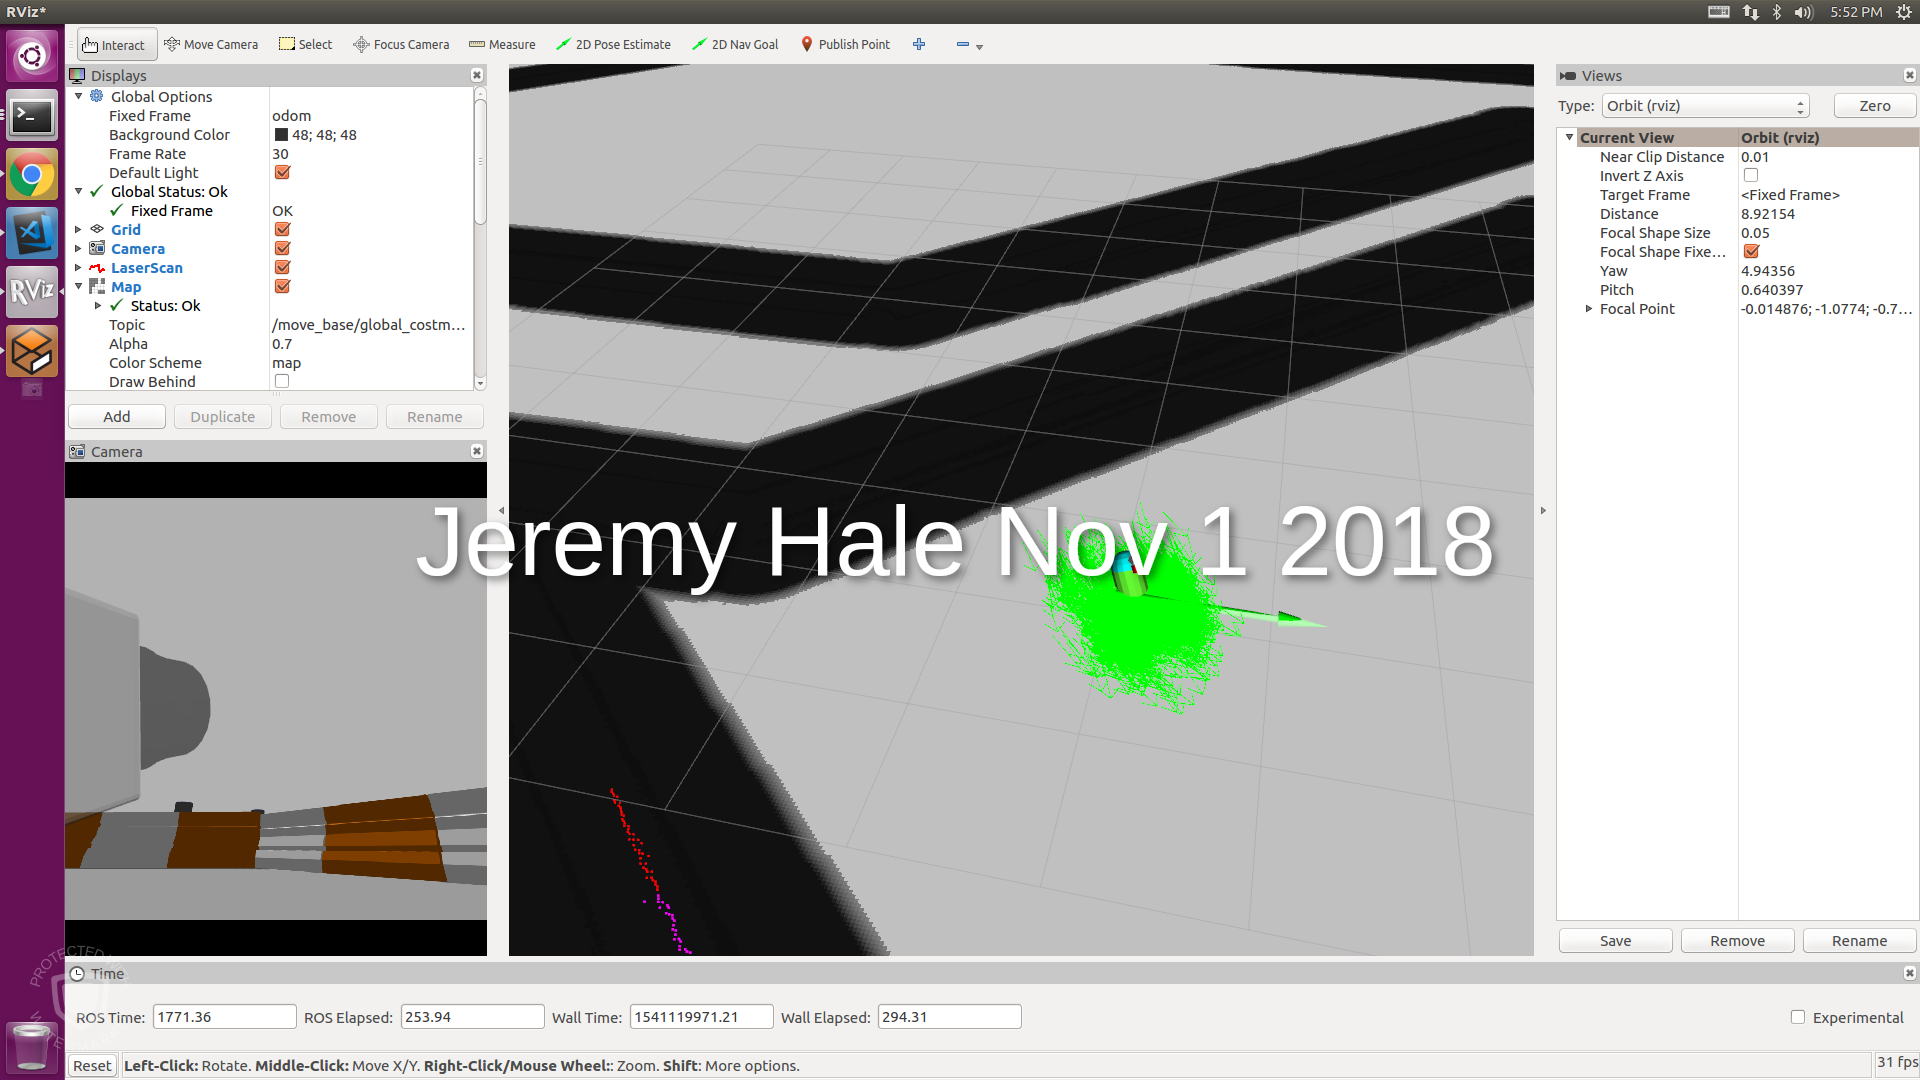
\includegraphics[width=\linewidth]{my_bot_rvis}
      \caption{My Robot}
      \label{fig:robot3}
\end{figure}

The command to launch the student robot world is:
\begin{lstlisting}[language=Bash]
roslaunch udacity_bot my_world.launch
\end{lstlisting}

For tuning both the costmap and the navigiation stack, the ROS documentation at the following URIs were used:

\url{http://wiki.ros.org/costmap\_2d}

\url{http://wiki.ros.org/navigation/Tutorials/RobotSetup}

The tuning parameters found in the documentation examples were used and found to be sufficient. Specifically, the update rate was lowered to 5 fps, the size of the local costmap was significantly reduced to 6x6, and the obstacle and raytrace range were set to the defaults of 2.5 and 3.0, respectively. The inflation radius was also set to 0.55 as per the example and proved to large enough that the robot would not become stuck on the wall but could still fit through narrow passages.

\subsection{Achievements}
Both models were able to navigate to the goal successfully.

% Robot Models
\subsection{Benchmark Model}
\subsubsection{Model design}
The benchmark model is a simple box with two driven wheels and two wheels for stability. The camera is front-mounted as is the laser scanner.
\subsubsection{Packages Used}
The packages used in the project should be specified as well as the topics received and published; the services it used and provided should also be addressed.


Packages:
\begin{itemize}
\item amcl
\item joint\_state\_publisher
\item move\_base
\item robot\_state\_publisher
\item tf
\end {itemize}
Topics (brief):
\begin{itemize}
\item /amcl
\item /joint\_states
\item /map
\item /move\_base/TrajectoryPlannerROS/cost\_cloud
\item /move\_base/TrajectoryPlannerROS/global\_plan
\item /move\_base/TrajectoryPlannerROS/local\_plan
\item /move\_base/current\_goal
\item /move\_base/global\_costmap/costmap
\item /move\_base/goal
\item /move\_base/local\_costmap/costmap
\item /move\_base\_simple/goal
\item /odom
\item /particlecloud
\item /tf
\item /udacity\_bot/camera1
\item /udacity\_bot/laser/scan
\end {itemize}

\subsubsection{Parameters}
As mentioned previously the costmap parameters were the same as the ROS tutorial example. The main parameters to change were reducing the local costmap size as opposed to the global map. Setting an inflation value so that the robot would not get stuck on the wall.
The AMCL parameters were also default parameters from
\url{http://wiki.ros.org/amcl}
. Only the tranform\_tolerance was increased to allow for delayed processing of the simulation.

\subsection{Personal Model}
% ditto
\subsubsection{Model design}
The student-defined model is an R2D2-type robot: 2 wheels drive the robot while 2 undriven wheels provide fore/aft stabilization. The camera is attached to the "head" of the robot and the laser scanner is floating above the head in order to keep it horizontal.
\subsubsection{Packages Used}
Same as benchmark.
\subsubsection{Parameters}
Same as benchmark.

\section{Results}
The robot meets the performance objective as it is only to reach the goal. No time limit was suggested or imposed.

The particle filter converges within a few second for the benchmark. The personal robot has a subjectively slightly worse localization. This is believed to be due to the non-smooth, jerky motion of the robot. The simulator causes jerky motion when in the physical world this would not happen.

In either case, the robot reaches the goal in under 30 seconds. There is a tendency for the robots to perform an "Austin Powers" manoeuvre where it goes back and forward between the two walls of corridor instead of heading straight down.

\subsection{Localization Results}
\subsubsection{Benchmark}
The images above show the clustering of green arrows indicating localization result.
\subsubsection{Student}
The images above show the clustering of green arrows indicating localization result.

\subsection{Technical Comparison} % only facts
The simpler benchmark robot performs better because it has smoother motion. The personal robot bounces fore/aft as it moves causing jitter in the laser scanner readings.

The parameters for both robots are the same and their times to the goal are not dissimilar. The R2D2-configuration is mechanically quite different from the benchmark, but due to the limits of the simulator, a rear stabilizing wheel had to be added. This made the two configurations more similar.

\section{Discussion}
The personal robot performed adequately reaching the goal slightly slower than the benchmark.

\subsection{Topics}
\begin{itemize}
\item Which robot performed better?
Benchmark
\item Why DID it performed better? (opinion)
The personal robot had a mechanical stability issues.
\item How would you approach the 'Kidnapped Robot' problem?
AMCL would work well for the kidnapped robot problem. Once deposited in the new location, the particle cluster would spread out randomly until the robot is able to re-localize itself. This was not tested but is the author's opinion.
\item IN What types of scenarios could localization be performed?
AMCL would work well in real life for situations where a well defined map exists.
\item Where would you use MCL/AMCL in an industry domain?
An industry example could be a warehouse. A warehouse is a fairly static well-defined environment that could be mapped. This technique would not work well for self-driving cars where the environment is constantly changing and large.

\end {itemize}

\section{Conclusion / Future work}
This project served as a toy example of tuning AMCL in a simulated environment. To that point, it was helpful to learn basic AMCL parameter tuning.

The techniques described above could be implemented easily on a hardware platform that supports Ubuntu linux. The hardware laser scanner and drive system would need plugins for ROS.

For future work, other sensors and drive systems could be explored such as the four wheel steering controller, etc.

\subsection{Modifications for Improvement}
Examples:
\begin{itemize}
\item Base Dimension
No change necessary.
\item Sensor Location
No change necessary.
\item Sensor Layout
Consider adding IMU.
\item Sensor Amount
Consider additional sensors.
\end{itemize}

\subsection{Hardware Deployment}
\begin{enumerate}
\item What would need to be done?
Mechanical construction, motors \& motor controllers, power supply and battery management, sensor hardware, single board computer.
\item Computation time/resource considerations?
There is a tradeoff in robot responsiveness (how fast it can process the update loop) and processing power.
\end{enumerate}



\bibliography{bib}
\bibliographystyle{ieeetr}

\end{document}